\subsection{Понятие анализатора сетевого трафика}

Анализатор трафика -- это программа или устройство, которое позволяет
анализировать сетевой трафик, проходящий через компьютерную сеть.
Анализаторы трафика, или снифферы, используются для мониторинга и
отслеживания сетевых активностей, обнаружения проблем и уязвимостей в сети,
а также для решения различных задач в области безопасности и
администрирования сети.


Основные составляющие анализатора трафика могут включать:
\begin{itemize}
    \item захват и анализ трафика: анализаторы трафика могут захватывать и
    анализировать сетевой трафик, передаваемый между компьютерами в сети;
    \item фильтрация трафика: анализаторы трафика могут фильтровать трафик,
    чтобы отображать только определенные типы сетевой активности, например,
    только HTTP-запросы;
    \item декодирование протоколов: снифферы могут декодировать различные
    протоколы, используемые в сети, чтобы обеспечить более подробное
    представление о том, какие данные передаются между компьютерами;
    \item графический интерфейс пользователя: анализаторы трафика могут
    предоставлять графический интерфейс пользователя (GUI) для удобного
    просмотра и анализа данных;
    \item возможность сохранения и экспорта данных: анализаторы трафика могут
    сохранять данные в различных форматах и экспортировать их для дальнейшего
    анализа или использования в других приложениях.
\end{itemize}

Анализаторы трафика являются неотъемлемой частью современных сетей
и позволяют обеспечивать безопасность, производительность и эффективность
работы сети. Они используются для мониторинга сетевых активностей,
обнаружения и предотвращения кибератак, анализа производительности и
оптимизации сетевых ресурсов. Снифферы могут быть полезными как для
крупных корпораций, так и для небольших организаций и даже домашних
пользователей, которые желают обеспечить безопасность своих домашних сетей
и улучшить их производительность.


Особенности анализаторов трафика:
\begin{itemize}
    \item безопасность: анализаторы трафика могут использоваться для
    обнаружения уязвимостей и атак в сети, а также для мониторинга соответствия
    сетевой политики и правил безопасности;
    \item администрирование сети: снифферы могут помочь в администрировании
    сети, позволяя управлять трафиком, оптимизировать производительность и
    обеспечивать соответствие сетевой политике;
    \item разработка и тестирование сетевых приложений: анализаторы трафика
    могут быть использованы для разработки и тестирования сетевых приложений,
    позволяя анализировать и отлаживать сетевой трафик, который передается
    между приложениями;
    \item решение проблем в сети: анализаторы трафика могут быть использованы
    для решения различных проблем в сети, таких как снижение
    производительности, отказы в работе и другие сбои;
    \item мониторинг сети: снифферы могут использоваться для мониторинга
    сетевых активностей, включая управление сетевой пропускной способностью,
    контроль за использованием ресурсов, управление сетевым доступом и т.д.;
    \item поддержка соответствия: анализаторы трафика могут помочь
    организациям удостовериться в соответствии различным регулирующим
    стандартам, например, стандартам PCI DSS, HIPAA и другим;
    \item улучшение производительности: анализаторы трафика могут помочь
    улучшить производительность сети, обеспечивая оптимальное использование
    ресурсов и предоставляя информацию для определения узких мест и проблем в
    сети;
    \item отладка сети: снифферы могут использоваться для отладки сетевых
    проблем, позволяя идентифицировать, где именно происходят ошибки и сбои в
    сети.
\end{itemize}


В целом, анализаторы трафика представляют собой важный инструмент
для мониторинга, анализа и управления сетевыми активностями, обеспечивая
безопасность, производительность и надежность сети. Основные функции и
возможности анализаторов трафика могут варьироваться в зависимости от
конкретных потребностей и сценариев использования, но в общем случае они
могут включать в себя следующие аспекты:
\begin{itemize}
    \item способность обрабатывать различные протоколы: анализаторы трафика
    должны иметь возможность обрабатывать различные протоколы, такие как
    HTTP, FTP, SMTP, TCP/IP, UDP, DNS и другие;
    \item функции фильтрации и поиска: снифферы должны иметь функции
    фильтрации и поиска, чтобы помочь пользователям находить необходимые
    данные и информацию в больших объемах трафика;
    \item режим захвата пакетов: анализаторы трафика должны иметь возможность
    захвата пакетов, передаваемых в сети, чтобы анализировать их содержимое и
    характеристики;
    \item отображение данных: анализаторы трафика должны предоставлять
    различные способы отображения данных, включая таблицы, графики и
    диаграммы, чтобы помочь пользователям визуализировать данные и
    информацию;
    \item удобный интерфейс: снифферы должны быть легкими в использовании и
    предоставлять удобный интерфейс для пользователя, чтобы снизить время
    обучения и повысить производительность;
    \item масштабируемость: анализаторы трафика должны иметь возможность
    масштабироваться для обработки больших объемов трафика и управления
    растущими сетевыми активностями;
    \item безопасность: анализаторы трафика должны быть безопасными для
    использования и обеспечивать конфиденциальность и защиту данных,
    передаваемых в сети;
    \item поддержка производительности: анализаторы трафика должны быть
    производительными и обеспечивать быстрое обнаружение и решение проблем в
    сети;
\end{itemize}


В зависимости от сценария использования, снифферы могут иметь
дополнительные функции, такие как анализ потока данных, декодирование
шифрованного трафика, определение топологии сети и др.



\begin{figure}[h!]
    \centering
    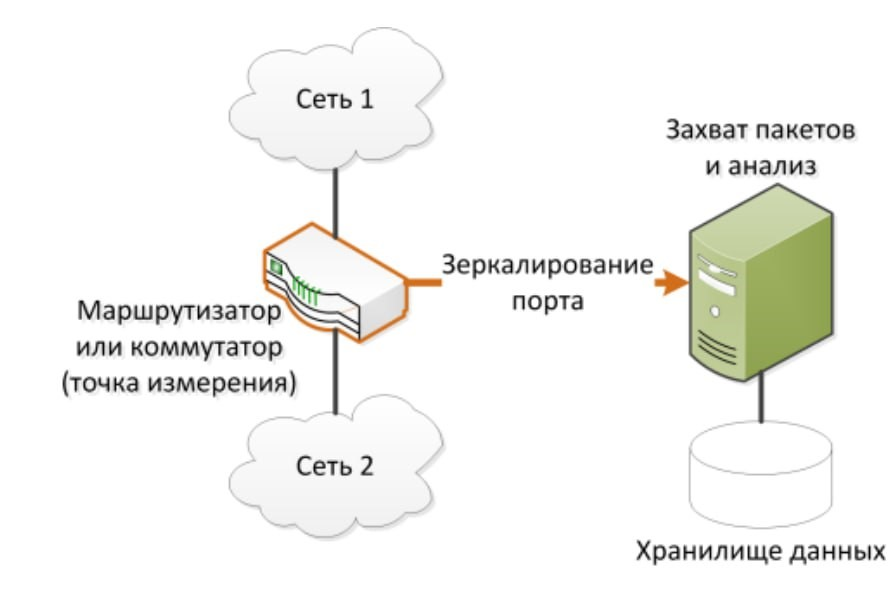
\includegraphics[width=0.85\linewidth]{\commonSecPathPrefix/sec_1/content/sniffer_work.jpg}
    \caption{Принцип работы анализатора сетевого трафика}
    \label{fig:snifwork}
\end{figure}



Принцип работы анализатора сетевого трафика заключается в захвате и
анализе пакетов, передаваемых в сети. Анализатор сетевого трафика может быть
реализован как программное или аппаратное средство и работать на уровне
сетевого интерфейса. Когда пакеты проходят через интерфейс, анализатор
сетевого трафика захватывает их и передает для анализа. После захвата пакетов,
анализатор сетевого трафика разбирает их на составляющие, такие как источник
и назначение, протокол, порт и другие атрибуты. Затем он анализирует
содержимое каждого пакета и использует специальные алгоритмы для
обнаружения аномальных и нежелательных пакетов\cite{unix_man}. Общая схема работы
анализатора сетевого трафика представлена на рисунке \ref{fig:snifwork}.


Сниффер может также использоваться для отображения информации о
сетевых узлах, скорости передачи данных, объеме передаваемых данных и
других метриках производительности сети.


Анализаторы сетевого трафика обладают рядом преимуществ, которые
делают их необходимыми инструментами для работы сетевых администраторов
и специалистов в области информационной безопасности. Это мощный
инструмент, который помогает эффективно управлять сетями и защищать их.
Снифферы обеспечивают надежную и безопасную работу сетей, а также
позволяют оптимизировать использование сетевых ресурсов и повысить
производительность приложений. Благодаря анализаторам сетевого трафика,
сетевые администраторы и специалисты по кибербезопасности могут быстро
реагировать на угрозы и проблемы в сети, что позволяет предотвратить
серьезные последствия для бизнеса и пользователя.

